\def\year{2020}\relax
%File: formatting-instruction.tex
\documentclass[letterpaper]{article} % DO NOT CHANGE THIS
\usepackage{aaai20}  % DO NOT CHANGE THIS
\usepackage{times}  % DO NOT CHANGE THIS
\usepackage{helvet} % DO NOT CHANGE THIS
\usepackage{courier}  % DO NOT CHANGE THIS
\usepackage[hyphens]{url}  % DO NOT CHANGE THIS
\usepackage{graphicx} % DO NOT CHANGE THIS
\urlstyle{rm} % DO NOT CHANGE THIS
\def\UrlFont{\rm}  % DO NOT CHANGE THIS
\usepackage{graphicx}  % DO NOT CHANGE THIS
\frenchspacing  % DO NOT CHANGE THIS
\setlength{\pdfpagewidth}{8.5in}  % DO NOT CHANGE THIS
\setlength{\pdfpageheight}{11in}  % DO NOT CHANGE THIS
%\nocopyright
%PDF Info Is REQUIRED.
% For /Author, add all authors within the parentheses, separated by commas. No accents or commands.
% For /Title, add Title in Mixed Case. No accents or commands. Retain the parentheses.
 \pdfinfo{
/Title (CS 494 Dissemination)
/Author (Timothy Player Smit Patel Josh Mandzak Doug Lowe)
} %Leave this	
% /Title ()
% Put your actual complete title (no codes, scripts, shortcuts, or LaTeX commands) within the parentheses in mixed case
% Leave the space between \Title and the beginning parenthesis alone
% /Author ()
% Put your actual complete list of authors (no codes, scripts, shortcuts, or LaTeX commands) within the parentheses in mixed case. 
% Each author should be only by a comma. If the name contains accents, remove them. If there are any LaTeX commands, 
% remove them. 
\usepackage{pgfplots}
\usepackage{tikz}
\usepackage{graphicx}
\usepackage{pgf-pie}

% DISALLOWED PACKAGES
% \usepackage{authblk} -- This package is specifically forbidden
% \usepackage{balance} -- This package is specifically forbidden
% \usepackage{caption} -- This package is specifically forbidden
% \usepackage{color (if used in text)
% \usepackage{CJK} -- This package is specifically forbidden
% \usepackage{float} -- This package is specifically forbidden
% \usepackage{flushend} -- This package is specifically forbidden
% \usepackage{fontenc} -- This package is specifically forbidden
% \usepackage{fullpage} -- This package is specifically forbidden
% \usepackage{geometry} -- This package is specifically forbidden
% \usepackage{grffile} -- This package is specifically forbidden
% \usepackage{hyperref} -- This package is specifically forbidden
% \usepackage{navigator} -- This package is specifically forbidden
% (or any other package that embeds links such as navigator or hyperref)
% \indentfirst} -- This package is specifically forbidden
% \layout} -- This package is specifically forbidden
% \multicol} -- This package is specifically forbidden
% \nameref} -- This package is specifically forbidden
% \natbib} -- This package is specifically forbidden -- use the following workaround:
% \usepackage{savetrees} -- This package is specifically forbidden
% \usepackage{setspace} -- This package is specifically forbidden
% \usepackage{stfloats} -- This package is specifically forbidden
% \usepackage{tabu} -- This package is specifically forbidden
% \usepackage{titlesec} -- This package is specifically forbidden
% \usepackage{tocbibind} -- This package is specifically forbidden
% \usepackage{ulem} -- This package is specifically forbidden
% \usepackage{wrapfig} -- This package is specifically forbidden
% DISALLOWED COMMANDS
% \nocopyright -- Your paper will not be published if you use this command
% \addtolength -- This command may not be used
% \balance -- This command may not be used
% \baselinestretch -- Your paper will not be published if you use this command
% \clearpage -- No page breaks of any kind may be used for the final version of your paper
% \columnsep -- This command may not be used
% \newpage -- No page breaks of any kind may be used for the final version of your paper
% \pagebreak -- No page breaks of any kind may be used for the final version of your paperr
% \pagestyle -- This command may not be used
% \tiny -- This is not an acceptable font size.
% \vspace{- -- No negative value may be used in proximity of a caption, figure, table, section, subsection, subsubsection, or reference
% \vskip{- -- No negative value may be used to alter spacing above or below a caption, figure, table, section, subsection, subsubsection, or reference

\setcounter{secnumdepth}{0} %May be changed to 1 or 2 if section numbers are desired.

% The file aaai20.sty is the style file for AAAI Press 
% proceedings, working notes, and technical reports.
%
\setlength\titlebox{2.5in} % If your paper contains an overfull \vbox too high warning at the beginning of the document, use this
% command to correct it. You may not alter the value below 2.5 in
\title{CS494 Final Project Dissemination Group II}
%Your title must be in mixed case, not sentence case. 
% That means all verbs (including short verbs like be, is, using,and go), 
% nouns, adverbs, adjectives should be capitalized, including both words in hyphenated terms, while
% articles, conjunctions, and prepositions are lower case unless they
% directly follow a colon or long dash
\author{Timothy Player, Doug Lowe, Josh Mandzak, Smit Patel \textsuperscript{\rm 1}\thanks{Dr. Alex Williams}\\ % All authors must be in the same font size and format. Use \Large and \textbf to achieve this result when breaking a line
\textsuperscript{\rm 1}University of Tennessee Knoxville\\ %If you have multiple authors and multiple affiliations
% use superscripts in text and roman font to identify them. For example, Sunil Issar,\textsuperscript{\rm 2} J. Scott Penberthy\textsuperscript{\rm 3} George Ferguson,\textsuperscript{\rm 4} Hans Guesgen\textsuperscript{\rm 5}. Note that the comma should be placed BEFORE the superscript for optimum readability
1520 Middle Drive\\
Knoxville, Tennessee  37996\\
tplayer@vols.utk.edu % email address must be in roman text type, not monospace or sans serif
}
 \begin{document}

\maketitle
\section{Introduction}
Introduction: Describe your use-case and why it matters. Summarize what you've done and learned.
Youtube Education is an add-on to the existing Youtube architecture which makes better youtube video recommendations based on the user’s preference. Youtube Education is designed to take in account the user’s mood through the use of a slider to see if they want more educational content suggested over entertaining content or vice versa. This agent accepts the user’s major, name of their classes , and allows for their syllabus in order to suggest more content closely related to their school work. The user can also control how much of the Youtube Education’s suggestions appear in their feed. Users can see more of a Youtube channel’s content in the Youtube Education’s suggestions by adding the channel to its own favorites list. 
	This system could have many uses in online education. The Youtube Education agent could help students stay focused on school while still using a great resource like Youtube. The system would be built on a platform that already has a large database of videos, but some recommendations are a problem. Youtube Education is an attempt to eliminate this weakness with better AI. In order to make the system easier to use, it can be partnered with Universities , so the students don’t have to enter all the information for their classes. The system was slowly improved using a need finding study and prototyping. 
	This development process was broken down into two different phases. The main purpose of the needfinding study is to look at users for design inspirations. Needfinding also helps with looking for surprises, finding the differences between what people say they do and what they actually do , and use users who are pushing the system to reveal needs before the mainstream. Prototyping is the second phase of the development of Youtube Education. In the prototyping phases the users are shown a lo-fi prototype of the agent, and they are asked what they think of the prototype. Using the feedback, the lo-fi prototype is improved in all needed places, and shown to the users until the desired product is created.  There is no limit to how many times this iteration is done even though Youtube Education used only one iteration.

\section{Need Finding}
For our needfinding we created 5 different personas to help us visualize how our product would affect the general population. We specifically wanted to hone in on the section of the population that is still undergoing education. Our first persona is Tiffany, a first year college student majoring in physics. She is a first generation college student and would like to learn more about her classes to accelerate her learning. She has developed poor study habits from online learning, she also falls asleep in class. We thought that our project would be useful in helping her fix her poor study habits and keep her attention so that she does not doze off in the middle of learning. Our second persona is Mark, a middle schooler with ADHD. He has issues focusing on schoolwork and spends his time binging videos on the internet and gaming with his friends. Our project could help him learn while still being as enjoyable as some of his other hobbies. Especially with the ability to intermingle our recommendations with the default recommendations we believe this project would be perfect for Mark. Our third persona is Jim, and undecided freshman who is unsure which major to pursue. He hasn't chosen a major because he lacks basic knowledge about the contents of each major. Jim wants to see more of what each major contains before making a decision. Our project could be used by Jim to help sooth his concerns about lacking knowledge. He could research easy to stomach information about multiple different majors to feel more educated on his decision. Our fourth persona is Alex, a 22-year-old neuroscience major in his senior year.  He works as a research assistant for his college and loves it, but is bogged down by loads of class work and constant tests. He would prefer to be working on his research then studying for his midterms. Our project could assist him by allowing him to study in a more enjoyable manner and possibly at a quicker pace so that he can return to his research work. Our final persona is different from the rest as she is supposed to be an “anti-persona” that we need to fix our project around. Her name is Helen and she is an elderly woman who is unsure of how to use the internet, but enjoys knitting. We created her to make sure that our project was clear enough that even people unsure about the internet might be able to use our project. Our project should be clear and straightforward enough for Helen to be able to look up educational knitting videos at her leisure. 
After we had created our personas we took our ideas and questions to real people and interviewed them about what they might want out of our project. Our first question was whether or not people would be willing to switch to our recommender from the current default recommender. We were met with a resounding distaste for the current recommender and a willingness to move to a new system. The second question was about where they find educational content currently. The responses were very uncertain with most people mentioning using youtube “Crash Courses” as well and generally searching for terms they were unsure of. One participant mentioned using channels they already know of, which prompted us to take that into account for our final prototype. For the third question we were unsure of the possible use of the purely educational portion of our project so we questioned whether or not the participants would use that section. The participants all responded that they would utilize that portion of the project if it was provided to them. Finally we asked what more they might want from our project. The main two answers that we received were that participants wanted an ability to mix the default recommender with our new one and an ability to adjust the length of the videos recommended. We took these opinions in consideration when designing the first prototype.

\section{Prototype}

From the information gleamed from need finding, we decided that tackling all the goals were too ambitious. So we decided to focus on 3 important base goals from Need Finding. Usability, integration, and user experience through the Lo-Fi Prototype. This is the default Youtube homepage$^{[\ref{fig:prototype0}]}$, which includes a small section labelled “Youtube Apps”. This section includes pages such as “Youtube Kids”, “Youtube Music”, etc. It followed that the recommender should be included there as it is an extension to the default Youtube homepage. Once clicked it would open up a menu with all of it’s options. Our recommendation engine would be visible here among the other apps. Once the application was clicked on it would open up a menu that allows the user to customize their recommendation experience. It will allow them to type in their major and/or classes with each choice being saved and removable. It would also allow the user to upload their syllabus for easy addition. It includes a slider that allows the user to decide how educational or entertaining their content suggestions are. As well as radio buttons that allow the user to set how much of their content should be based on our educational recommendations. Finally it has a save and cancel button that allows the user to save their changes or disregard them.

\begin{figure}[h]
    \centering
    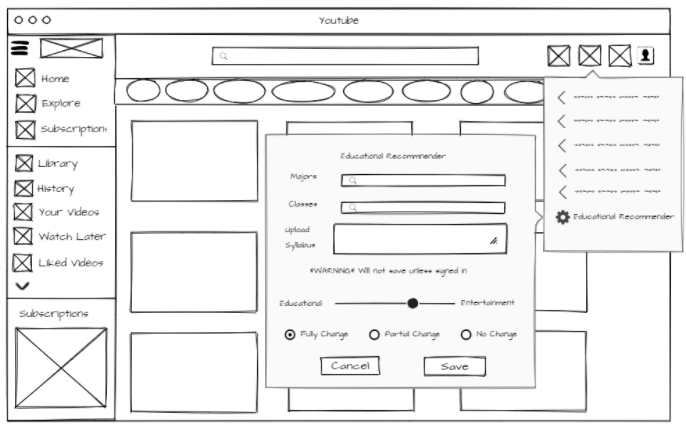
\includegraphics[width=8cm, hieght=8cm]{AuthorKit20/LaTeX/prototype0.PNG}
    \caption{Initial Prototype}
    \label{fig:prototype0}
\end{figure}

 After the changes were made, the homepage would look like this$^[]$. People were unaware of or did not the use YouTube Apps button. People were unclear on what the partial, full, and no change buttons did. People instinctively put in class number rather than name on occasion. People wanted options to favorite channels. People wanted to use this for multiple classes, not just one. Changes from first the iteration.We iterate on the initial design and found the users were confused by the buttons so we replaced it with a slider. 

Moved from YouTube Apps to its own button, indicated by book icon. Changed “change buttons” to the percent videos replaced slider. Added blue question mark that shows text box describing the field when hovered over/clicked on for classes field and percent videos replaced field.

\begin{figure}[h]
    \centering
    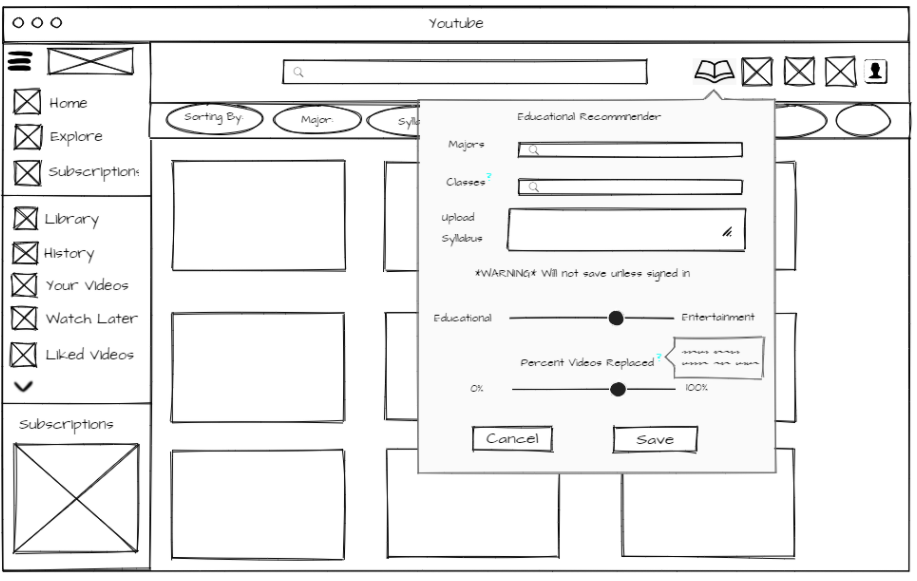
\includegraphics[width=8cm, hieght=8cm]{AuthorKit20/LaTeX/prototype.PNG}
    \caption{Final Prototype}
    \label{fig:prototype}
\end{figure}
\section{Future Work}
Describe what could follow your prototype work.
This research project is by no means the end of the line for the idea of a YouTube Education possibility in the real world. This project focused mainly on discovering the wants and needs of everyday YouTube users when it came to an idea such as YouTube Education. Thus, the next logical step in the process is to build a functioning prototype that can be deployed on the official YouTube website.
This next step in the process would likely begin with constructing the algorithm used to suggest videos to users. This would take a team of software engineers focusing on a few key aspects. The team would likely begin with gathering a dataset of all the information mentioned in the prototype we presented. Necessary information to include in this dataset would be major, classes, syllabi, an integer value containing the education to entertainment percentage, and a list of favorited channels per user. In an ideal scenario, an initial database used for testing would contain multiple users with combinations of this information per user.
Once the dataset had been created, the engineers could then create an algorithm based on these parameters that performs the actual task of creating a list of recommended videos. Multiple implementations could be created, each evaluated by the engineers themselves or by focus groups to see how well the algorithm performed to user expectations. Additional research projects could be launched here to have one last test of desirability before production.
A last step in this process of future work would be to launch the agent to production and assess the YouTube community’s opinion on it.


\section{Contributions}

\end{document}
